\apendice{Documentación de usuario}

\section{Introducción}

En esta sección se enumeran los requisitos que debe cumplir el usuario para poder usar la aplicación, se explica el proceso de instalación y se ofrece un manual de usuario completo para aprender a usarla. 

\section{Requisitos de usuarios}

Para poder instalar y usar la aplicación el dispositivo del usuario debe complir los siguientes requisitos: 

\begin{itemize}
	\item Contar con una versión de Android 6 (\textit{Marshmallow}) o superior, la cual corresponde con la API 23 de Android. 
	\item Permitir la instalación de aplicaciones de orígenes desconocidos~\cite{origenesdesconocidos}. Para ello: 
	\begin{enumerate}
		\item Ir a los ajustes del dispositivo. 
		\item A la opción de \textbf{Seguridad} o \textbf{Privacidad} según la versión. 
		\item Activar la opción \textbf{Orígenes desconocidos}. 
	\end{enumerate}
	\item Contar con conexión a internet. 
\end{itemize}

Además, para poder entrar en la aplicación deberá tener un usuario y una contraseña asignados. 

\section{Instalación}

La instalación de una aplicación Android es muy sencilla. Solo es necesario pasar el archivo \textbf{SmartBeds.apk} al sistema de ficheros del dispositivo Android y seleccionarlo. En caso de tener activada la opción de permitir la instalación de aplicaciones de orígenes desconocidos y contar con el suficiente espacio de almacenamiento la aplicación se instalará automáticamente. 

Se recuerda que el archivo .apk se encuentra en el repositorio del proyecto\footnote{\url{https://github.com/aog0036/TFG-SmartBeds}}, en la ruta \textbf{/android/app/release}.

\section{Manual del usuario}

En esta sección se ofrece un manual para el uso de todas las funcionalidades de la aplicación. 

\subsection{Iniciar sesión}

Al ejecutar la aplicación desde el dispositivo Android la primera pantalla que se muestra es la de Iniciar Sesión. En esta pantalla se nos pide un nombre de usuario y una contraseña para acceder al sistema. Se debe: 

\begin{enumerate}
	\item Introducir el nombre de usuario. 
	\item Introducir la contraseña. 
	\item Pulsar el botón <<Iniciar sesión>>. 
\end{enumerate}

En caso de haber introducido valores correctos se accederá a la siguiente pantalla, en caso contrario un cuadro de diálogo nos indicará que el usuario o la contraseña introducidos no son correctos. 

Si el usuario introducido tiene un rol de administrador la siguiente pantalla será el \textbf{Menú de administración}. Si tiene un rol de usuario la siguiente pantalla será la de \textbf{Visualización de camas}. 

\begin{figure}[H]
	\centering
	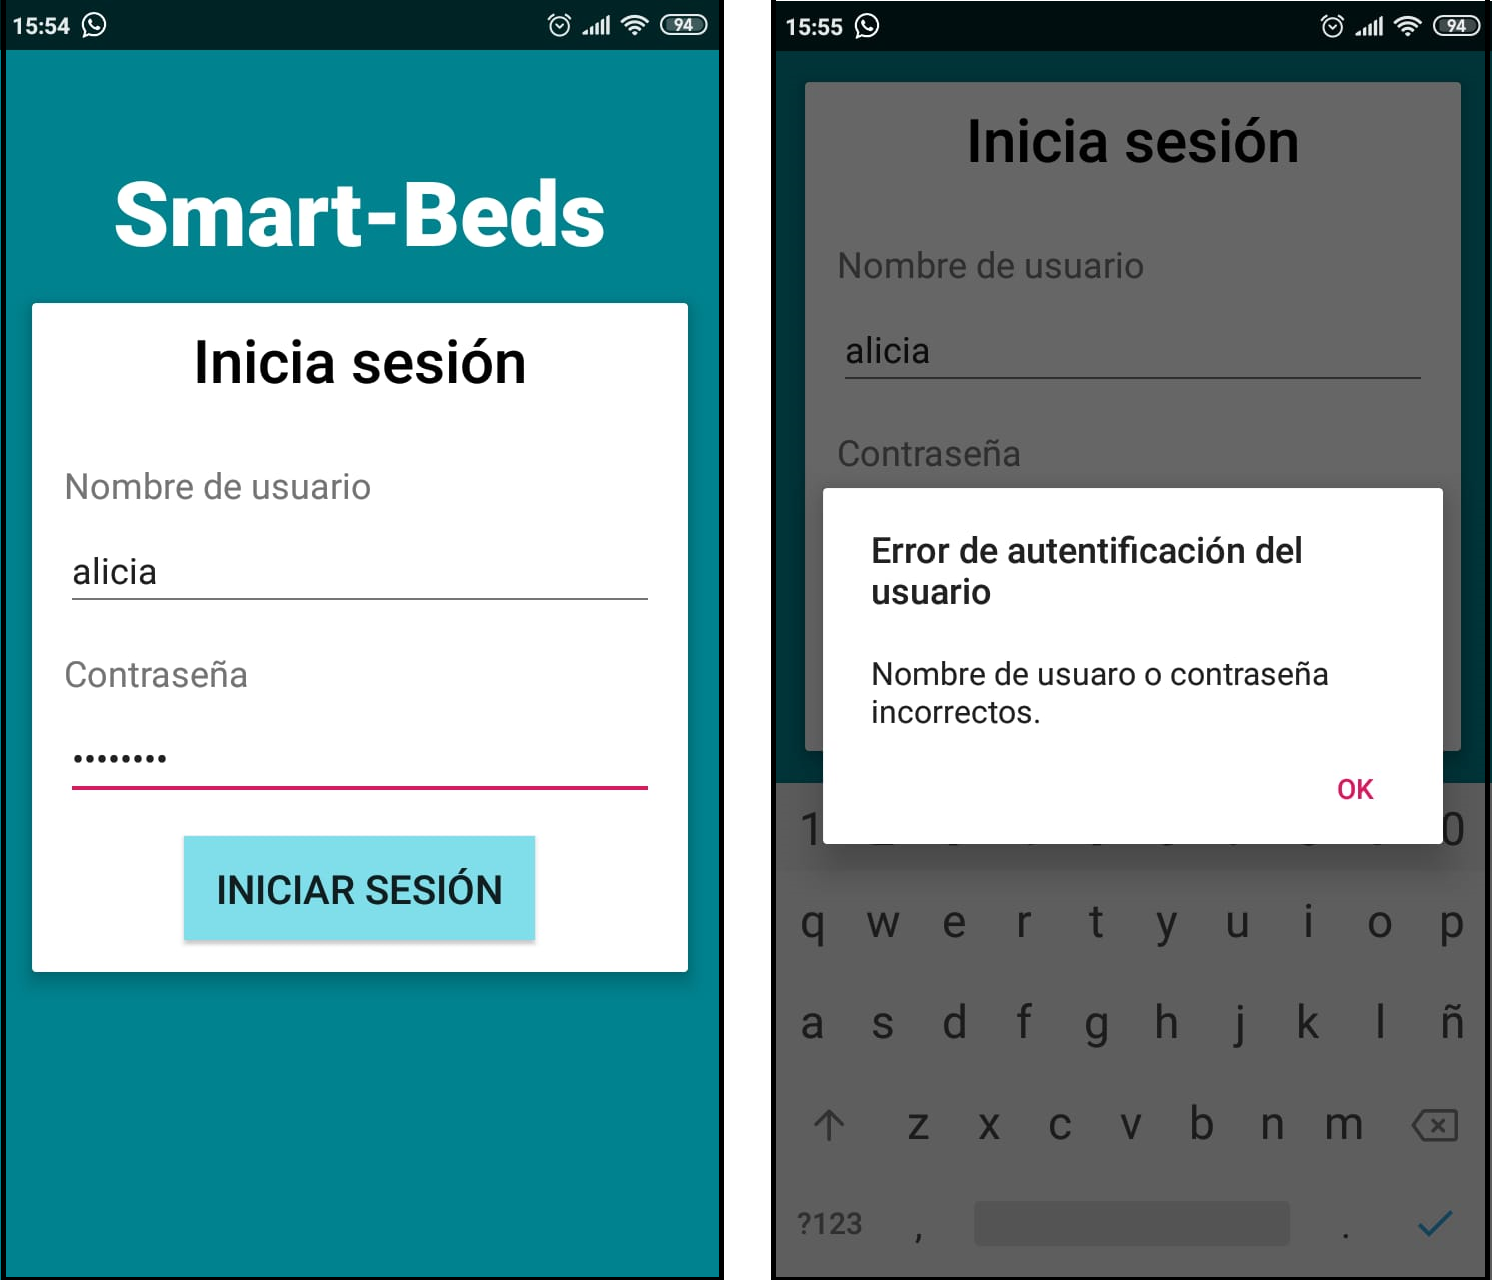
\includegraphics[width=0.7\textwidth]{../img/iniciasesion.png}
	\caption{Iniciar sesión.}
	\label{fig:iniciasesion}
\end{figure}

\subsection{Menú de administración}

Este menú solo está disponible si el usuario tiene un rol de administrador. En él puedes escoger a qué función de la aplicación deseas acceder: \textbf{Gestión de usuarios}, \textbf{Gestión de camas} o \textbf{Visualización de camas}. 

\begin{figure}[H]
	\centering
	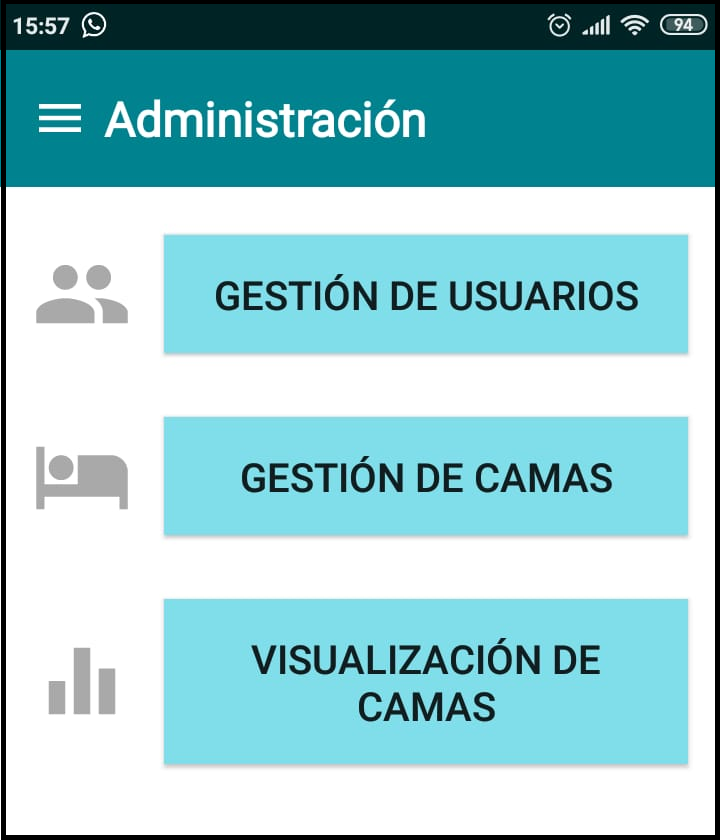
\includegraphics[width=0.4\textwidth]{../img/menudeadministracion.png}
	\caption{Menú de administración.}
	\label{fig:menudeadministracion}
\end{figure}

\subsection{Gesión de usuarios}

Esta pantalla solo está disponible si el usuario tiene un rol de administrador. En esta pantalla se muestra una lista de todos los usuarios registrados en el sistema. Al mantener pulsado uno queda seleccionado y se muestran las opciones disponibles: \textbf{Cambiar contraseña} y \textbf{Eliminar}.

\begin{itemize}
	\item Si escogemos \textbf{Cambiar contraseña} se muestra una pantalla donde debemos introducir dos veces la nueva contraseña y pulsar el botón <<Cambiar contraseña>>.
	\item Si escogemos \textbf{Eliminar} aparece un cuadro de diálogo preguntando al usuario si desea eliminar de forma permanente al usuario seleccionado. 
	\item Para \textbf{añadir un nuevo usuario} al sistema debemos pulsar en el símbolo <<+>> en la esquina inferior derecha de la pantalla, la cual nos llevará a una pantalla donde deberemos introducir el nombre de usuario y la contraseña del nuevo usuario, y pulsar el botón <<Añadir usuario>>. 
\end{itemize}  

\begin{figure}[H]
	\centering
	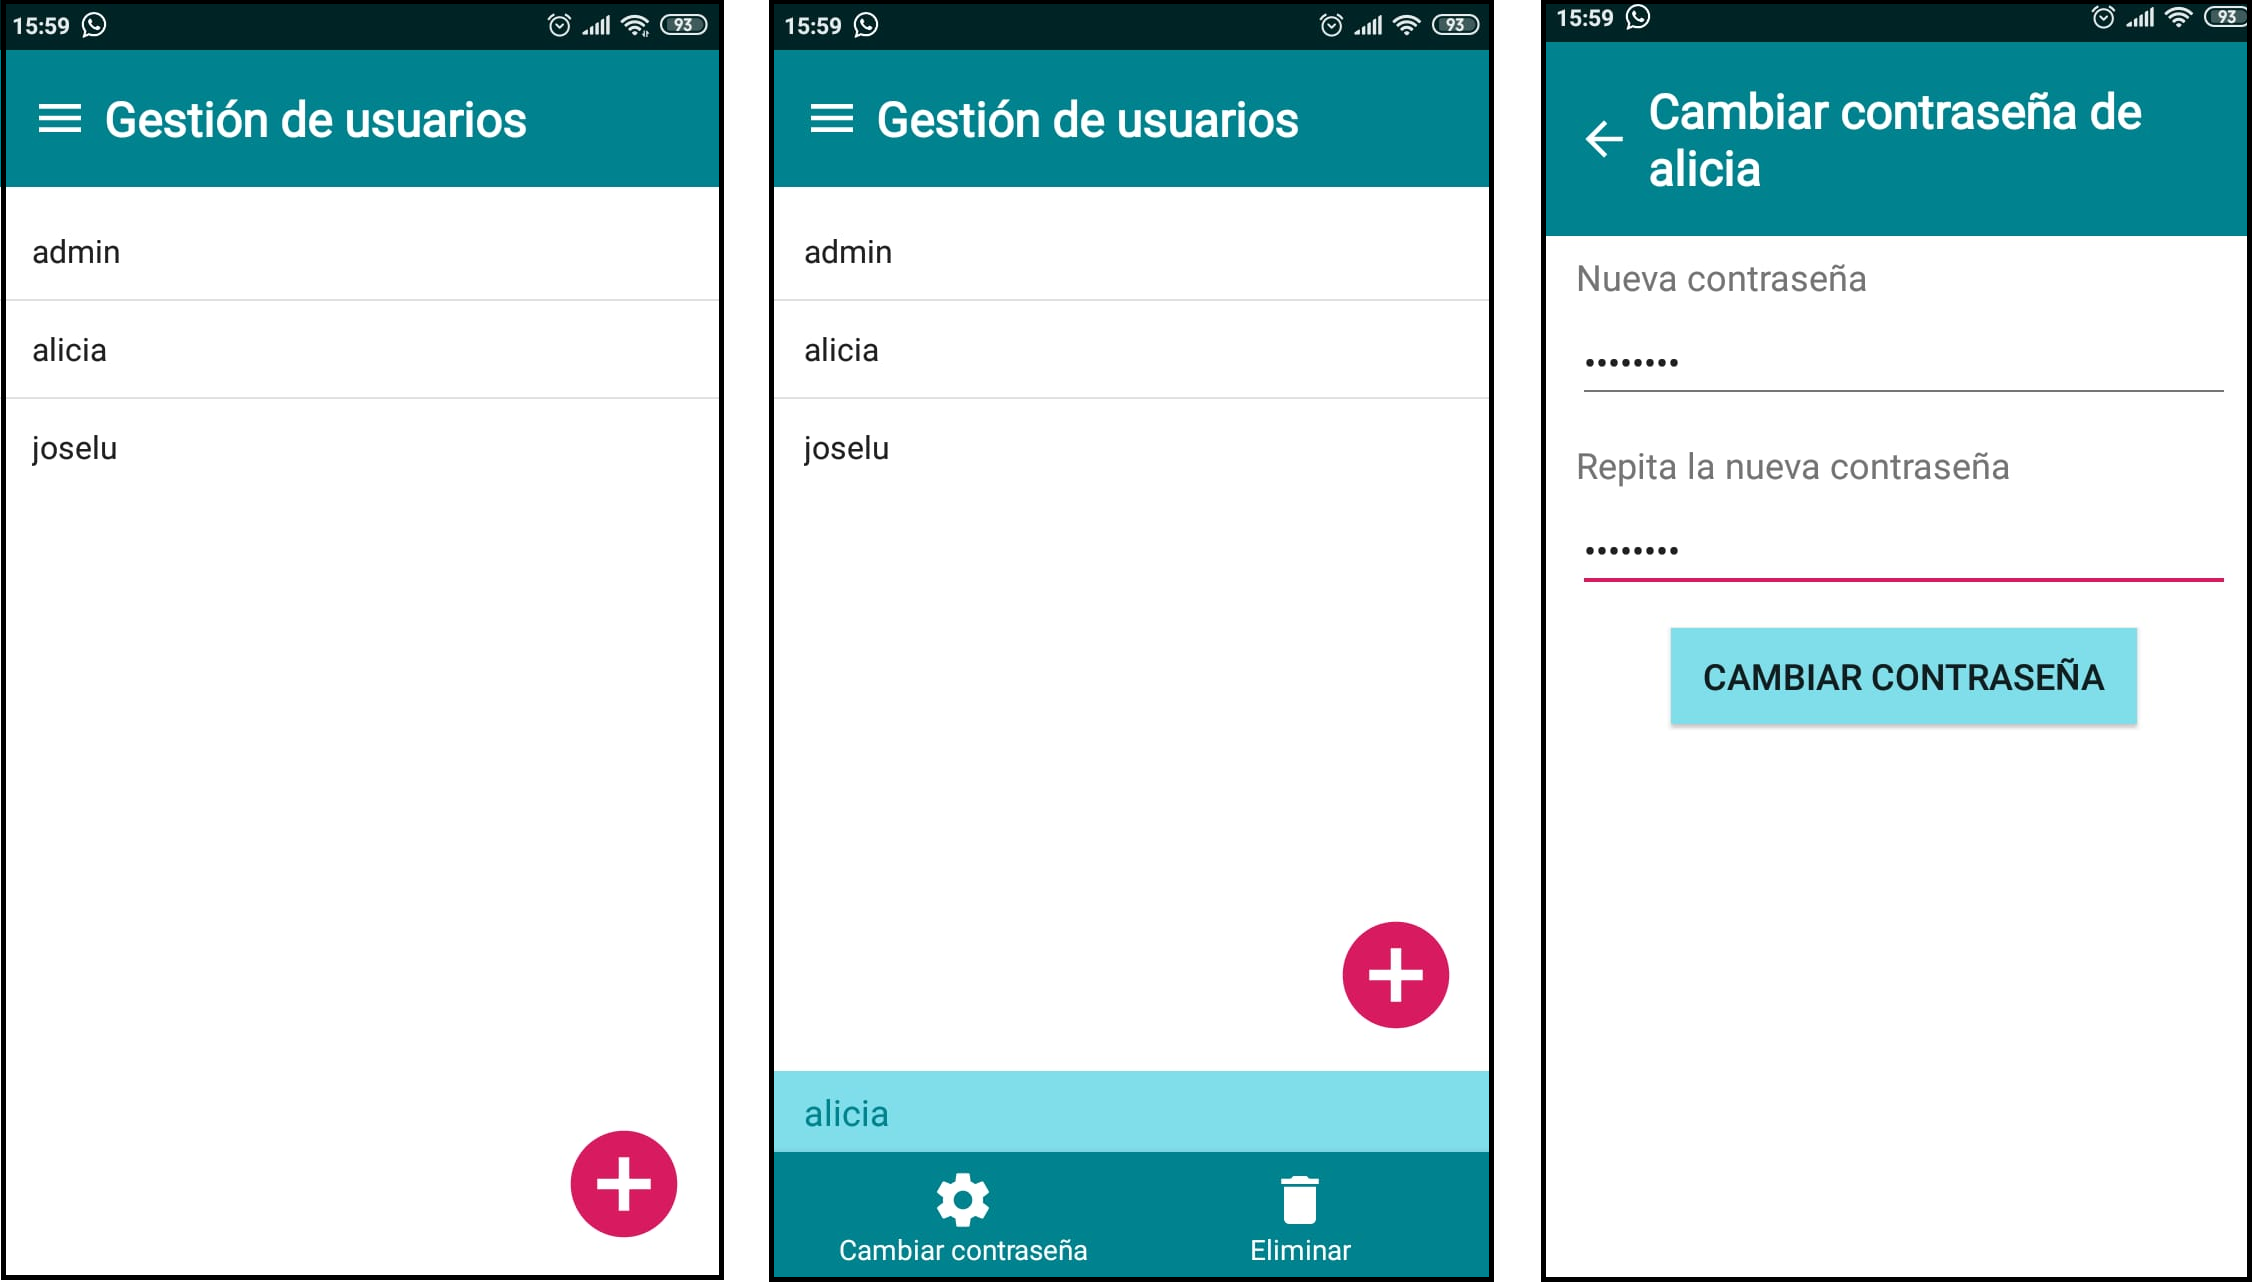
\includegraphics[width=1\textwidth]{../img/gestiondeusuarios.png}
	\caption{Gestión de usuarios, cambiar contraseña.}
	\label{fig:gestiondeusuarios}
\end{figure}

\begin{figure}[H]
	\centering
	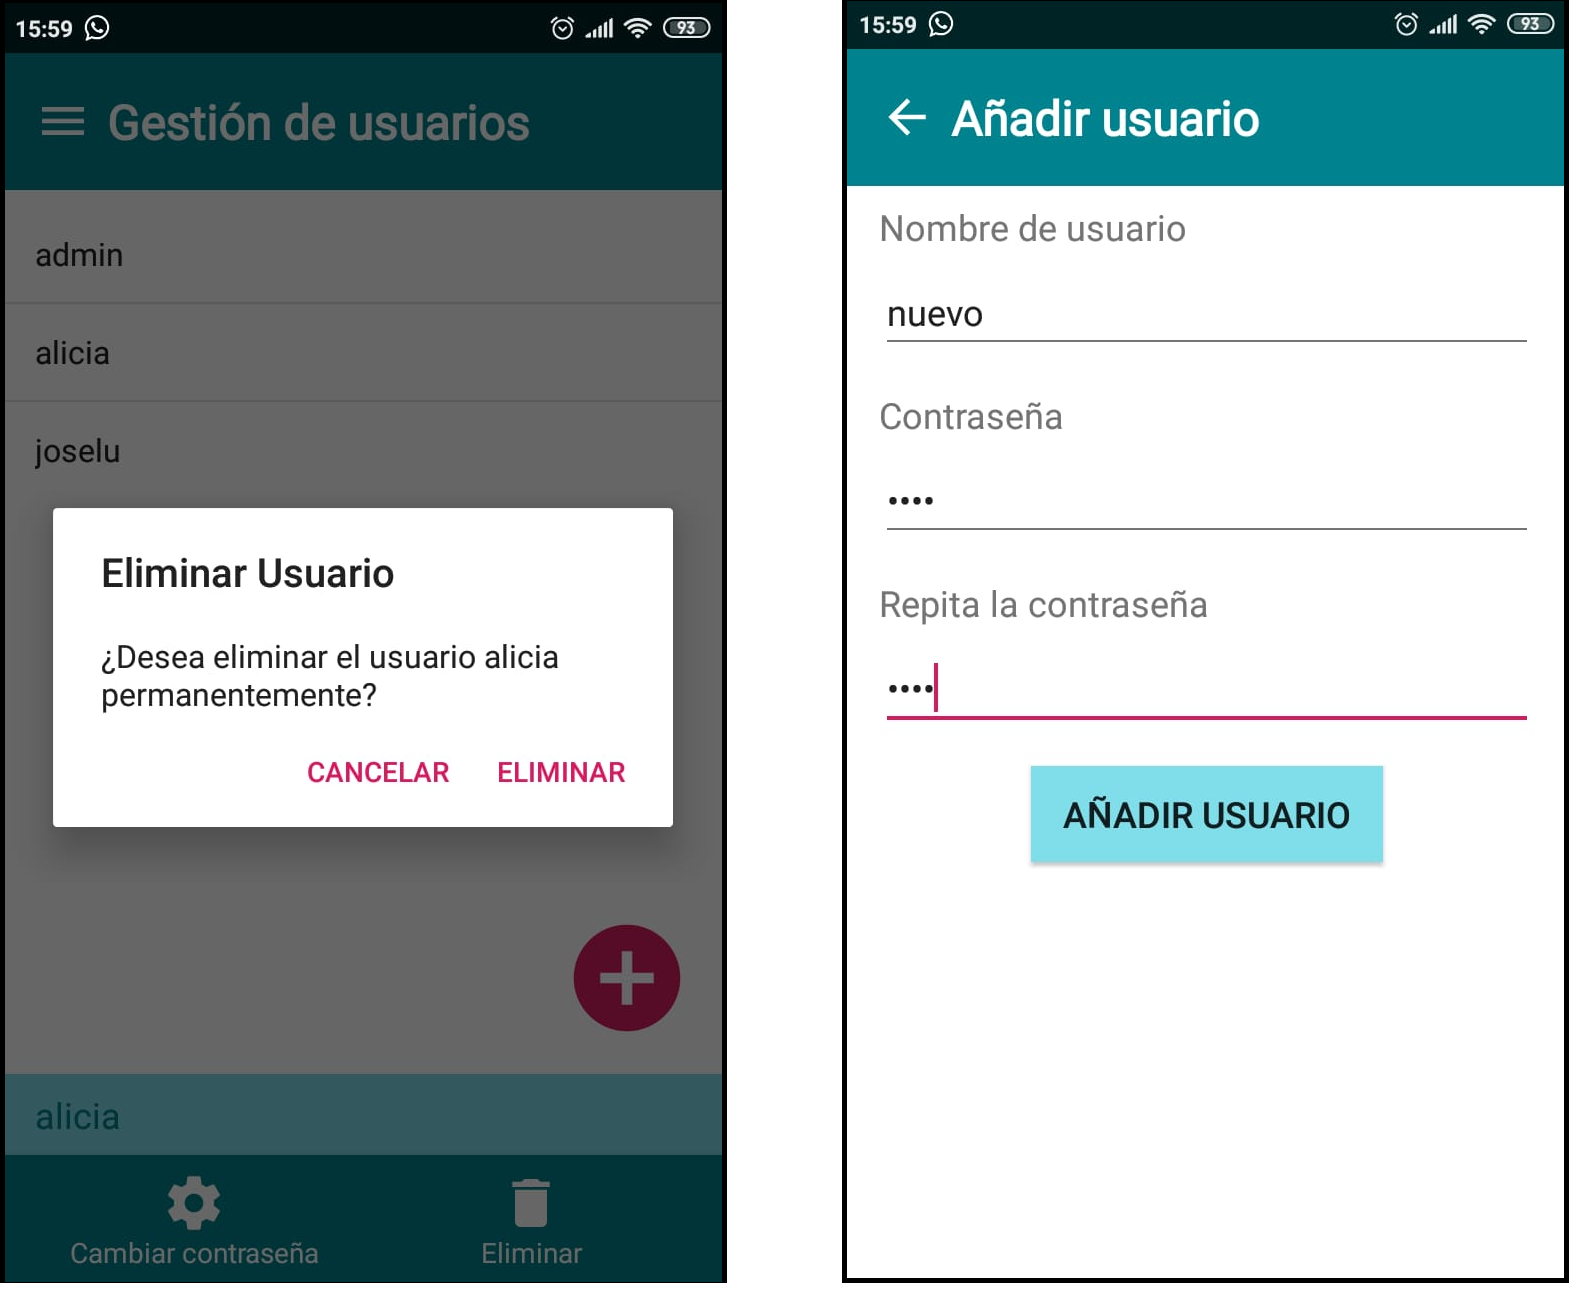
\includegraphics[width=0.7\textwidth]{../img/eliminaranadir.png}
	\caption{Gestión de usuarios, eliminar y añadir usuarios.}
	\label{fig:eliminaranadir}
\end{figure}

\subsection{Gestión de camas}

Esta pantalla solo está disponible si el usuario tiene un rol de administrador. En esta pantalla se muestra una lista de todas las camas registradas en el sistema. Al mantener pulsada una queda seleccionada y se muestran las opciones disponibles: Modificar, Eliminar y Asignar usuarios.  

De estas tres funciones, en esta versión de la aplicación solo está disponible la de \textbf{Asignar usuarios}, al seleccionar el resto solo se muestra un cuadro de diálogo informativo. Seleccionar la opción <<Asignar usuarios>> lleva a una pantalla donde se muestra una lista de todos los usuarios del sistema. En esta lista se pueden marcar aquellos que se desea que puedan ver la cama seleccionada y desmarcar los que no. 

\begin{figure}[H]
	\centering
	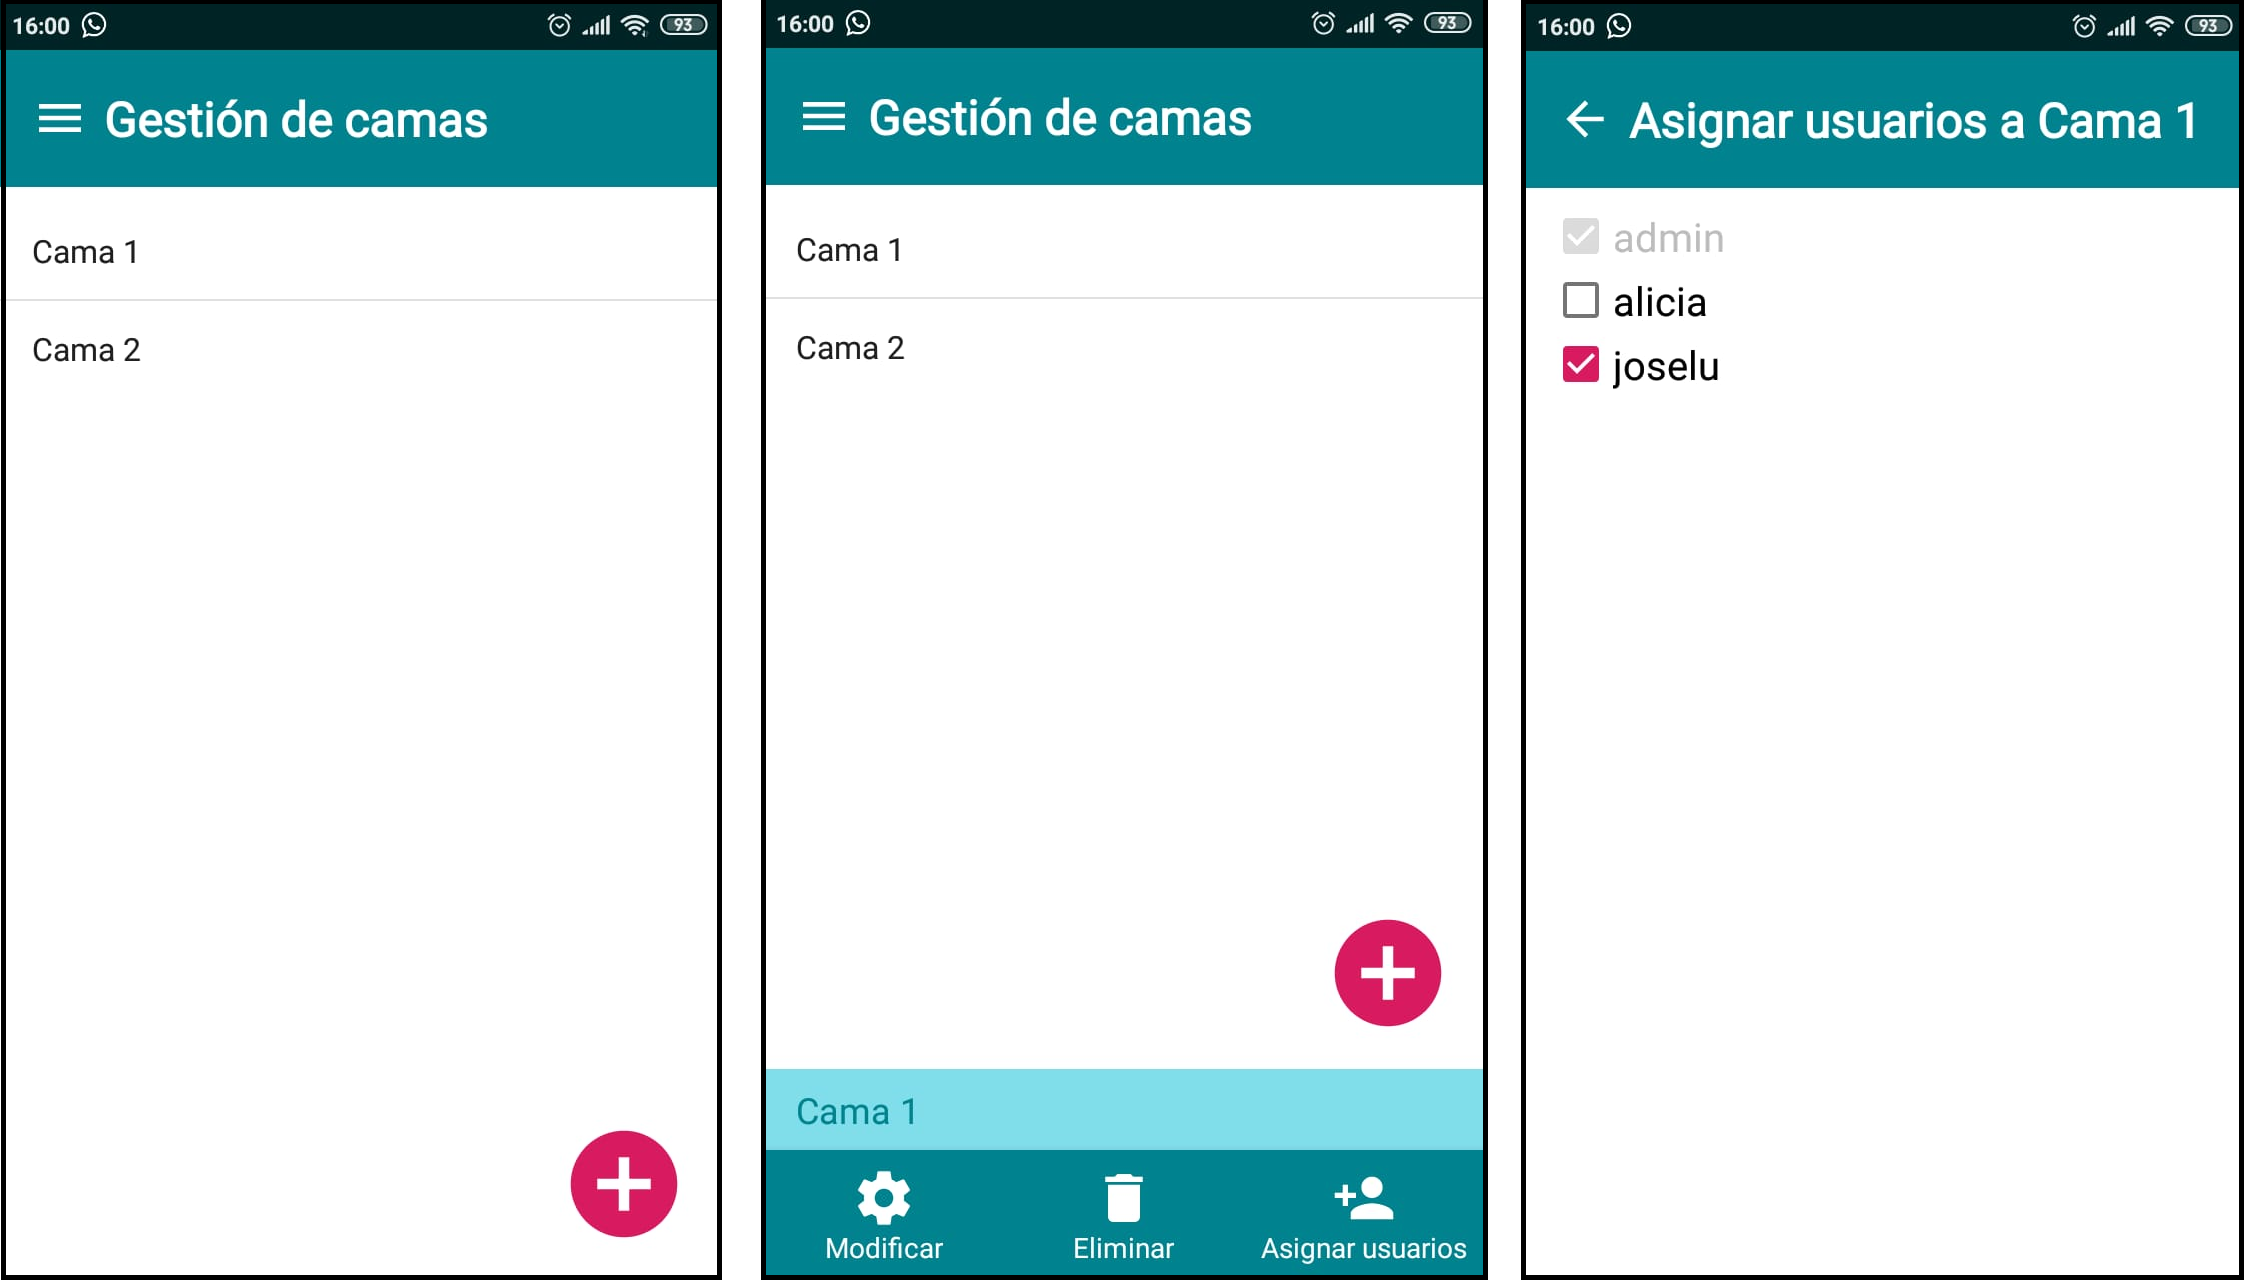
\includegraphics[width=0.9\textwidth]{../img/gestiondecamas.png}
	\caption{Gestión de camas, asignar usuarios.}
	\label{fig:gestiondecamas}
\end{figure}

\subsection{Visualización de camas}

Esta pantalla está disponible para usuarios con un rol de administrador y con un rol de usuario normal. Los administradores tendrán visibles todas las camas del sistema, los usuarios normales solo aquellas que el administrador les haya asignado. 

La pantalla muestra una lista de camas junto con el estado del paciente asociado en tiempo real (dormido, crisis epiléptica, cama vacía o datos insuficientes). Al pulsar una de las camas se accede a la pantalla de \textbf{Visualización de los datos de una cama en tiempo real}. 

\begin{figure}[H]
	\centering
	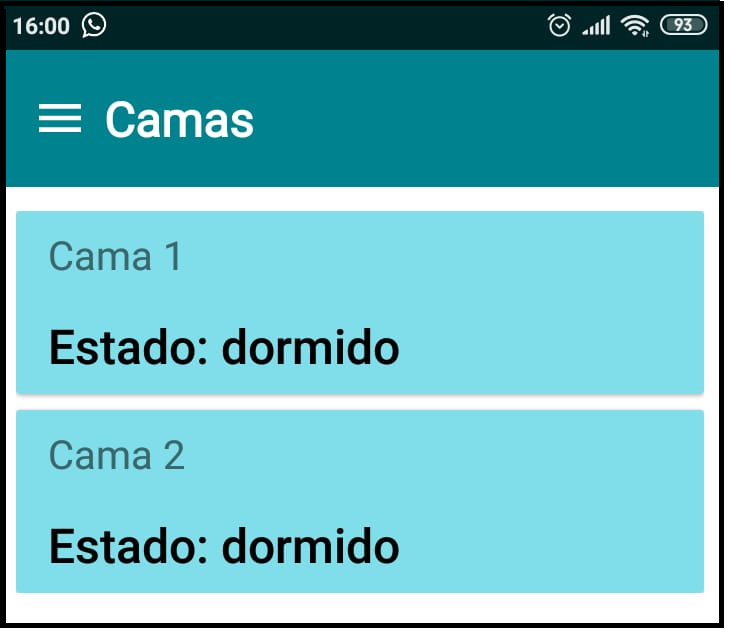
\includegraphics[width=0.4\textwidth]{../img/visualizaciondecamas.png}
	\caption{Visualización de camas.}
	\label{fig:visualizaciondecamas}
\end{figure}

\subsection{Visualización de los datos de una cama en tiempo real}

Esta pantalla está disponible para usuarios con un rol de administrador y con un rol de usuario normal. Un usuario normal solo podrá acceder a la pantalla asociada a una cama concreta si tiene permisos para visualizar esa cama. 

Esta gráfica se divide en tres pestañas que contienen distintas gráficas cuyos datos se actualizan en tiempo real: 

\begin{itemize}
	\item La primera contiene una gráfica con la probabilidad de que el paciente esté sufriendo una crisis epiléptica. 
	\item La segunda contiene una gráfica que muestra una línea de datos por cada sensor de presión instalado en el interior del colchón. 
	\item La tercera contiene cinco gráficas relativas a las constantes vitales del paciente: 
	\begin{itemize}
		\item Frecuencia cardíaca (pulsaciones/minuto)
		\item Frecuencia respiratoria (respiraciones/minuto)
		\item Volumen sistólico (mililitros)
		\item Variabilidad de la frecuencia cardíaca (milisegundos)
		\item Tiempo entre pulsaciones (milisegundos)
	\end{itemize}
\end{itemize}

\begin{figure}[H]
	\centering
	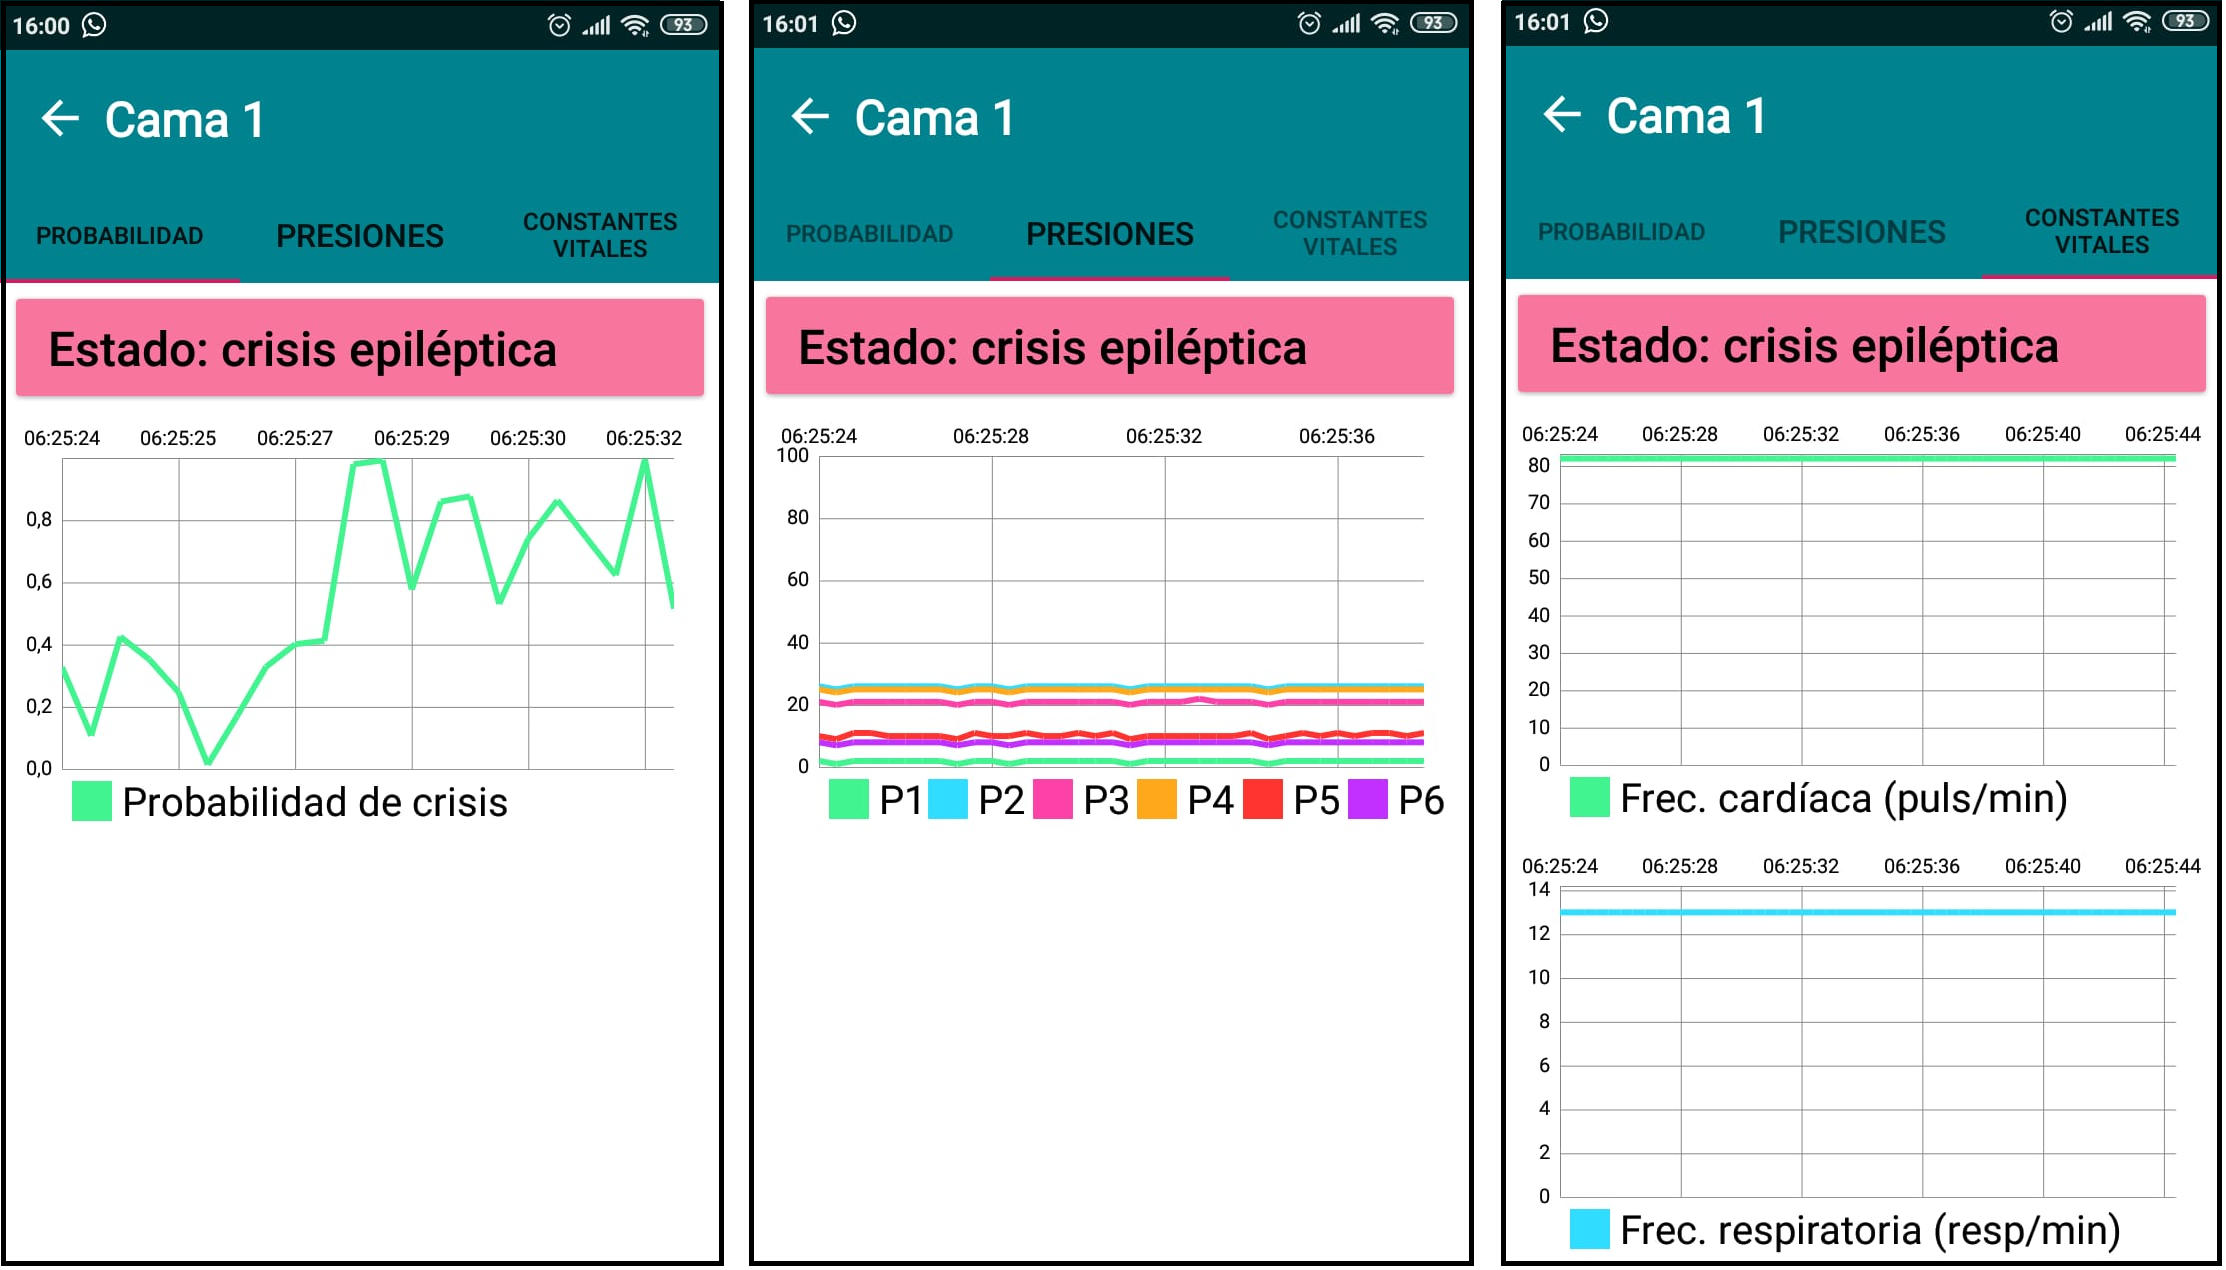
\includegraphics[width=0.9\textwidth]{../img/datoscama.png}
	\caption{Visualización de los datos de una cama en tiempo real.}
	\label{fig:datoscama}
\end{figure}

\subsection{Menú de navegación}

En las pantallas en las que se puede ver un icono de menú en la esquina superior izquierda es posible desplegar un menú de navegación pulsando el icono o deslizando el dedo por la pantalla de izquierda a derecha. Como se aprecia en la figura~\ref{fig:menunavegacion}, este menú contiene opciones distintas si se trata de un usuario con rol de administrador o un usuario normal. 

Para un usuario administrador incluye las mismas opciones que para un usuario normal y adicionalmente, las opciones del menú de administración. De esta forma se proporciona al administrador otra forma de navegar por la aplicación. Además de estas opciones se muestran tres más: \textbf{Modificar contraseña}, \textbf{Acerca de} y \textbf{Cerrar sesión}. La opción <<Cerrar sesión>> devuelve al usuario a la página inicial, las otras dos opciones llevan a sus respectivas pantallas.  

\begin{figure}[H]
	\centering
	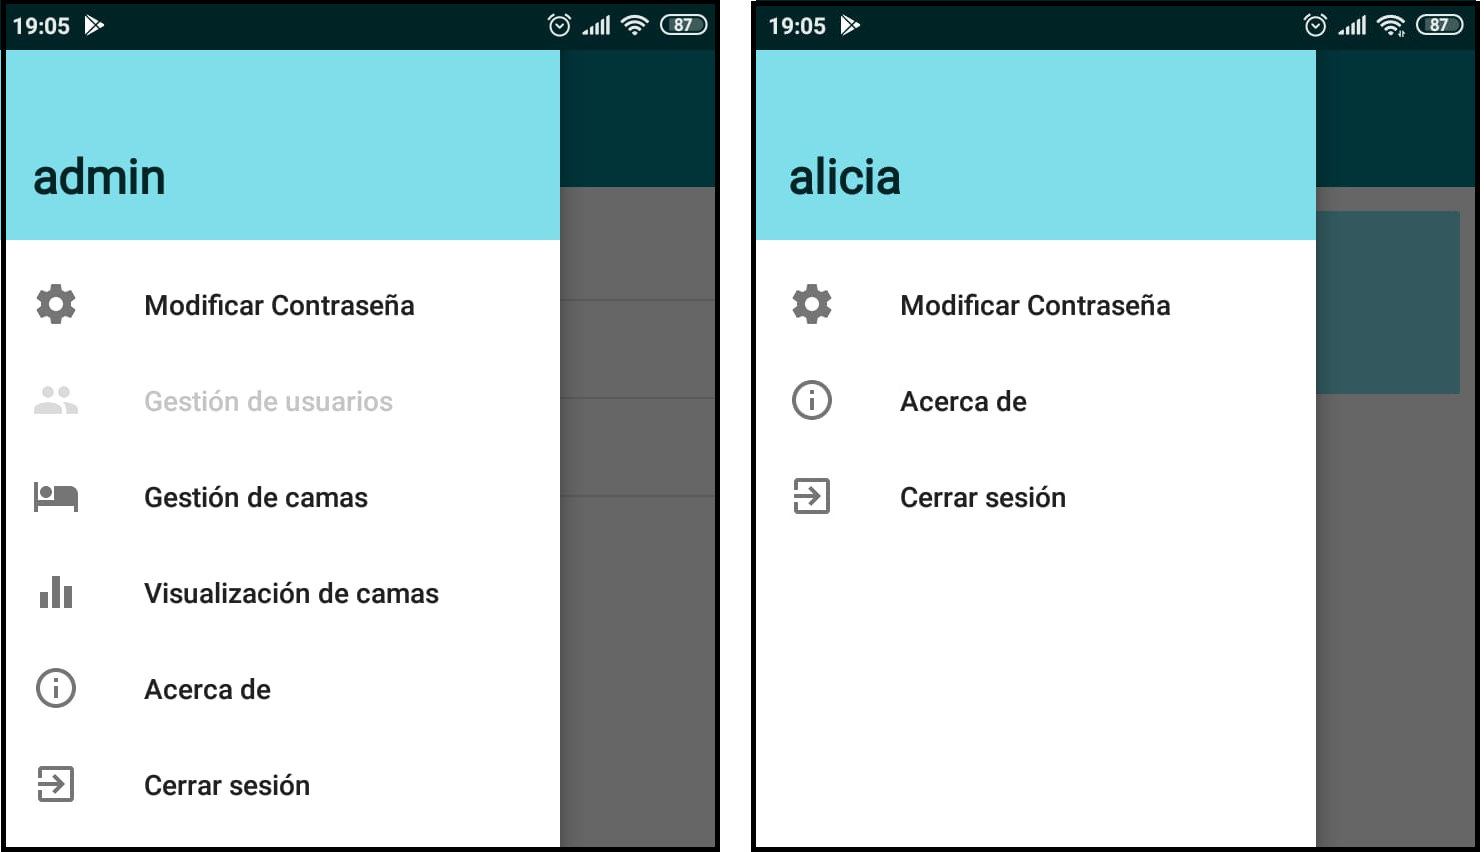
\includegraphics[width=0.7\textwidth]{../img/menunavegacion.png}
	\caption{Menú de navegación para un administrador y para un usuario normal.}
	\label{fig:menunavegacion}
\end{figure} 

\subsection{Modificar contraseña}

Hemos visto que el administrador puede cambiar la contraseña de cualquier usuario del sistema, pero mediante la opción Modificar contraseña del menú de navegación se permite cambiar la contraseña del usuario que se encuentra identificado en el sistema. En esta pantalla se debe introducir una vez la antigua contraseña, dos veces la contraseña por la que se desea modificar y pulsar el botón <<Cambiar contraseña>>. 

\begin{figure}[H]
	\centering
	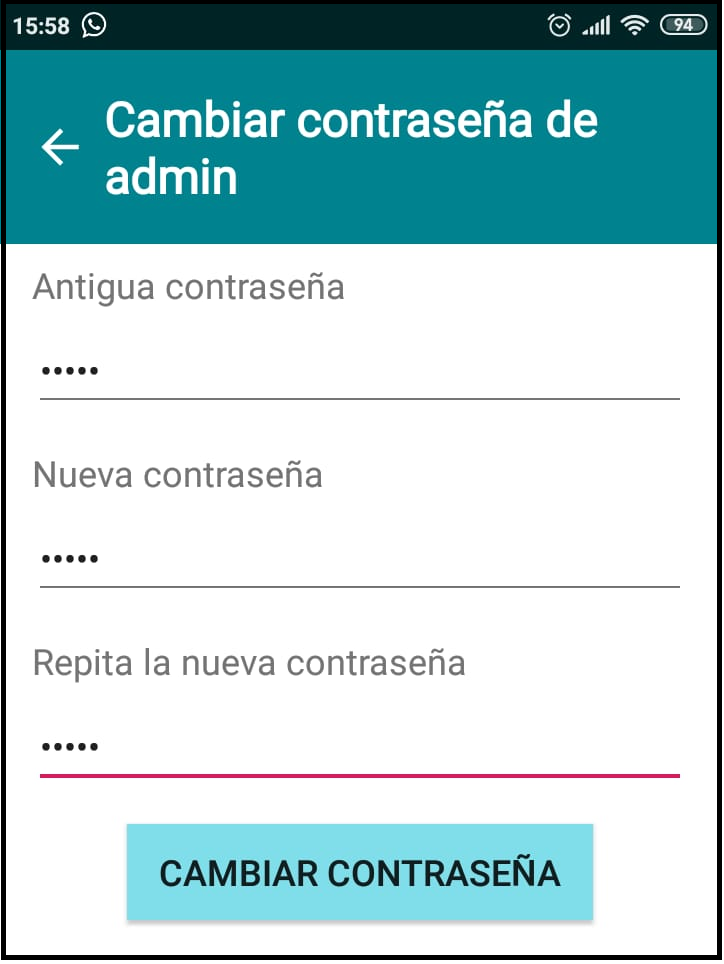
\includegraphics[width=0.4\textwidth]{../img/cambiarcontrasena.png}
	\caption{Modificar contraseña.}
	\label{fig:cambiarcontrasena}
\end{figure} 

\subsection{Acerca de}

TODO


